
%(BEGIN_QUESTION)
% Copyright 2008, Tony R. Kuphaldt, released under the Creative Commons Attribution License (v 1.0)
% This means you may do almost anything with this work of mine, so long as you give me proper credit

The Rockwell/Allen-Bradley MicroLogix 1000 programmable logic controller (PLC) can handle up to four analog input signals: two with a 0-10 V maximum range and two with a 0-20 mA maximum signal range.  This PLC's analog input terminal block looks like this (the internal resistors are shown inside the PLC box):

$$\includegraphics[width=15.5cm]{i04522x01.eps}$$

Sketch the appropriate wiring to connect one of these loop-powered transmitters to a voltage input and the other to a current input (IA/0 and IA/2) on the PLC.  Sketch a precision resistor in the appropriate location to convert the first transmitter's 4-20 mA current signal into a 1-5 V voltage signal appropriate for the voltage input channel.

\vskip 10pt

A schematic diagram showing the general connection scheme for a loop-powered 4-20 mA transmitter is shown here.  The transmitter acts as a {\it current regulator} to establish circuit current at a value depending on the physical variable being measured (e.g. pressure, temperature, level, flow, etc.):

$$\includegraphics[width=15.5cm]{i04522x03.eps}$$

\vfil 

Note: the two ``IA SHD'' terminals are provided for cable shield conductor attachment.  You may ignore cable shield wires and these terminals for simplicity's sake.

\underbar{file i04522}
\eject
%(END_QUESTION)





%(BEGIN_ANSWER)

This is a graded question -- no answers or hints given!
 
%(END_ANSWER)





%(BEGIN_NOTES)

As always, a good problem-solving strategy for sketching a pictorial circuit diagram is to first draw a clean schematic diagram of that circuit.  You were given a sample diagram showing one transmitter connected to the source and resistor, but you could easily add the second transmitter and second resistor to the same schematic in order to provide yourself with a plan to work from.  Note that loop-powered transmitters act as electrical {\it loads} rather than as true current sources, which is why you see current (conventional flow) entering the positive terminal and exiting from the negative terminal of each one:

$$\includegraphics[width=15.5cm]{i04522x04.eps}$$

The next order of business is determining what kind of signal each PLC input expects to receive.  Here we see a great disparity in input resistance between the two sets of input channels: the upper pair are high-resistance inputs (210 k$\Omega$) while the lower pair are low-resistance inputs (160 $\Omega$).  From this we should recall the ideal input resistance of voltmeters and ammeters: voltmeters should ideally have very high (infinite) resistance, while ammeters should ideally have negligible resistance.  This is to ensure minimum loading of the signal under test by the meter.

Both of our process transmitters have 4-20 mA current outputs which means one of them will naturally interface with the PLC current input channel (low-resistance) while the PLC voltage input channel will need some help in order to interpret a 4-20 mA current signal.

In order to get a 1-5 VDC signal range from the 4-20 mA transmitter, we need a resistance value of 250 $\Omega$.  Since each voltage input channel has an internal resistance value of 210 k$\Omega$, this means we must connect a 250.3 $\Omega$ resistor in parallel with the voltage input terminals in order to arrive at 250 ohms.  Truth be told, connecting a precision 250 $\Omega$ resistor to those terminals will be close enough to 250 ohms for all but the most precise applications.

\vskip 10pt

\filbreak

Following this revised schematic diagram, we may sketch the following solution:

$$\includegraphics[width=15.5cm]{i04522x02.eps}$$

\filbreak

Another good problem-solving technique to apply here is sketching arrows showing where conventional flow (current) enters and exits each component, based on its voltage polarity and its identity as either a source or a load.  Once these arrows are sketched, it becomes a trivial matter to connect tip-to-tail to form a series circuit:

$$\includegraphics[width=15.5cm]{i04522x05.eps}$$

{\it Any} connections that put the tip of one arrow connecting the tail of another will form a valid series circuit!


%INDEX% Pictorial circuit review (4-20 mA loop)

%(END_NOTES)


